\documentclass[11pt,a4paper]{article}

% --- Packages ---
\usepackage[utf8]{inputenc}
\usepackage[T1]{fontenc}
\usepackage{geometry}
\geometry{margin=0.8in}
\usepackage{hyperref}
\usepackage{graphicx}
\usepackage{booktabs}
\usepackage{array}
\usepackage{titlesec}
\usepackage{fancyhdr}
\usepackage{enumitem}
\usepackage{caption}
\usepackage{xcolor}
\usepackage{float}
\usepackage[most]{tcolorbox} % For professional frames

% --- Path Configuration ---
\graphicspath{{explination-diagram/}}

% --- Colors ---
\definecolor{primary}{HTML}{2563EB} % Tailwind blue-600
\definecolor{secondary}{HTML}{DBEAFE} % Tailwind blue-100
\hypersetup{
    colorlinks=true,
    linkcolor=primary,
    filecolor=magenta,      
    urlcolor=primary,
}

% --- Header and Footer ---
\setlength{\headheight}{14.5pt}
\pagestyle{fancy}
\fancyhf{}
\fancyhead[L]{\textbf{InjuryAssist}}
\fancyhead[R]{\thepage}
\fancyfoot[C]{\footnotesize \textperiodcentered\ 2026}

% --- Formatting ---
\titleformat{\section}{\normalfont\Large\bfseries\color{primary}}{\thesection}{1em}{}
\titleformat{\subsection}{\normalfont\large\bfseries\color{primary}}{\thesubsection}{1em}{}
\setlist[itemize]{noitemsep, topsep=2pt}

% --- Custom Command for Models ---
\newtcolorbox{modelbox}[1]{
    colback=white,
    colframe=primary!50,
    fonttitle=\bfseries,
    title=#1,
    sharp corners,
    boxrule=0.5pt,
    halign=center,
    valign=center,
    drop shadow
}

% --- Document Information ---
\begin{document}

% --- Professional Header ---
\begin{center}
    {\Huge \textbf{Software Requirements Specification}} \\
    \vspace{0.3cm}
    {\LARGE \textbf{InjuryAssist: Patient-Doctor Management Platform}} \\
    \vspace{0.6cm}
    \textbf{Prepared by:} Ahmed Moumen , Ali Osman \\
    \vspace{0.2cm}
    \textbf{Organization:} Arab Academy for Science, Technology \& Maritime Transport \\
    \textbf{Course Lecturer:} Dr/Ammar Ibrahim \textperiodcentered\ \textbf{Repository:} \href{https://github.com/Ali-CTRLS/cyber--repo}{GitHub} \\
    \vspace{0.4cm}
    \hrule
\end{center}

\tableofcontents
\newpage

% --- Section 1: Introduction ---
\section{Introduction}

\subsection{Purpose}
The purpose of this document is to define the Software Requirements Specification (SRS) for the \textbf{InjuryAssist Secure Patient-Doctor Injury Management Platform}. This document outlines the functional and non-functional requirements of the system, acting as a comprehensive guide for developers, cybersecurity evaluators, and stakeholders. It covers the entire scope of the InjuryAssist system, including secure user authentication, injury submission, doctor matching, and AES-256-GCM file encryption for medical reports.

\subsection{Document Conventions}
This document follows the IEEE formatting standard for SRS. Priority levels (High, Medium, Low) are assigned to system features to guide the development phases. Requirements are identified by unique tags (e.g., \texttt{REQ-SEC-1}).

\subsection{Intended Audience and Reading Suggestions}
This document is intended for:
\begin{itemize}
    \item \textbf{Developers \& Security Analysts:} To understand technical implementations, cryptographic strategies, and write test cases.
    \item \textbf{Project Managers:} To track feature development and define milestones.
    \item \textbf{Stakeholders \& Academics:} To ensure alignment with cybersecurity coursework and objectives.
\end{itemize}
\textit{Suggestion:} Readers are advised to start with Section 2 to grasp the overall system context before proceeding to detailed security constraints in Sections 3 and 4.

\subsection{Product Scope}
InjuryAssist is a cybersecurity-focused medical platform designed to streamline injury assessments by connecting patients with specialized doctors. Its primary objectives include automating doctor matching, scheduling appointments, and ensuring absolute data privacy through secure authentication, role-based access control (RBAC), and at-rest encryption (AES-256-GCM) of sensitive medical reports.

\subsection{References}
\begin{itemize}
    \item \textbf{UML Model Output:} \texttt{explination-diagram/}
    \item \textbf{Frameworks:} Python 3.9+, Flask 3.1.1, cryptography 44.0.0
\end{itemize}

% --- Section 2: Overall Description ---
\section{Overall Description}

\subsection{Product Perspective}
InjuryAssist is a self-contained web application. It serves as an academic demonstration of applied cybersecurity in healthcare software, centralizing patient tracking, doctor scheduling, and encrypted report generation into a single secure environment.

\subsection{Product Functions}
Based on the system's architecture, InjuryAssist provides the following major functions:
\begin{itemize}
    \item \textbf{Authentication \& Security:} Secure login, registration via PBKDF2 hashing, Flask-Login session management, and Flask-WTF CSRF protection.
    \item \textbf{Role-Based Access Control (RBAC):} Strict separation between Patient workflows and Doctor dashboards.
    \item \textbf{Patient Flow:} Submission of injuries, dynamic doctor matching based on body part, and appointment booking.
    \item \textbf{Doctor Dashboard:} Managing incoming appointments, confirming/canceling slots, and generating patient reports.
    \item \textbf{Cryptographic Storage:} Uploading and encrypting medical reports using AES-256-GCM prior to disk storage, with seamless on-the-fly decryption upon authorized download.
\end{itemize}

\subsection{User Classes and Characteristics}
\begin{itemize}
    \item \textbf{Patient:} Active users who submit injuries, browse matched doctors, book appointments, and download their decrypted medical reports. Needs a simple, trustworthy interface.
    \item \textbf{Doctor:} Medical professionals who manage their availability, review patient injuries, and securely upload diagnosis/treatment reports.
\end{itemize}

\subsection{Operating Environment}
\begin{itemize}
    \item \textbf{Platform:} Web-based (responsive UI via Tailwind CSS).
    \item \textbf{Server:} Python Flask application running on local port 5001.
    \item \textbf{Database:} SQLite with Flask-SQLAlchemy ORM (file-based).
\end{itemize}

\subsection{Design and Implementation Constraints}
\begin{itemize}
    \item \textbf{Data Security:} Medical files must be encrypted at rest using AES-256-GCM. Passwords must be hashed via Werkzeug's \texttt{generate\_password\_hash}.
    \item \textbf{Framework Restrictions:} No complex frontend frameworks (e.g., React/Angular); system strictly uses Jinja2 templates and Tailwind CDN for simplicity.
    \item \textbf{Database Restrictions:} Zero-configuration SQLite environment to ensure portability.
\end{itemize}

\subsection{User Documentation}
A comprehensive \texttt{README.md} and \texttt{instructions.md} provide setup steps, default credentials, and an architectural roadmap.

% --- Section 3: External Interface Requirements ---
\section{External Interface Requirements}

\subsection{User Interfaces}
\begin{itemize}
    \item \textbf{Patient Dashboard:} Displays injury history, upcoming appointments, and accessible medical reports.
    \item \textbf{Doctor Dashboard:} Displays appointment requests and provides interfaces for file uploads and report drafting.
    \item \textbf{Consistency:} Unified "White + Blue" design system indicating a clean, professional medical environment.
\end{itemize}

\subsection{Software Interfaces}
\begin{itemize}
    \item \textbf{Database API:} SQLAlchemy ORM interfacing with SQLite.
    \item \textbf{Cryptography API:} Python \texttt{cryptography} library utilized for AES GCM algorithms.
\end{itemize}

\subsection{Communications Interfaces}
\begin{itemize}
    \item \textbf{HTTP/HTTPS:} Standard web communication protocols.
    \item \textbf{Local Storage:} Direct disk I/O operations strictly confined to the \texttt{storage/reports/} directory for encrypted payloads.
\end{itemize}

% --- Section 4: System Features ---
\section{System Features}

\subsection{Authentication and RBAC}
\textbf{Priority: High.} The system must protect endpoints using session-based authentication and prevent privilege escalation.
\begin{itemize}[label=--]
    \item \texttt{REQ-AUTH-1}: Implement secure hashing (PBKDF2) for all user passwords.
    \item \texttt{REQ-AUTH-2}: Separate blueprints for \texttt{/patient} and \texttt{/doctor} routes with strict \texttt{@login\_required} decorators.
    \item \texttt{REQ-AUTH-3}: Prevent direct object references; users cannot view reports not assigned to them.
\end{itemize}

\subsection{Injury \& Appointment Management}
\textbf{Priority: High.} Patients must be matched accurately with doctors.
\begin{itemize}[label=--]
    \item \texttt{REQ-FLOW-1}: System auto-suggests doctors based on the selected body part of the injury.
    \item \texttt{REQ-FLOW-2}: Appointments follow a strict state machine: PENDING $\rightarrow$ CONFIRMED $\rightarrow$ COMPLETED.
    \item \texttt{REQ-FLOW-3}: Only pending appointments can be canceled by patients.
\end{itemize}

\subsection{Secure Report Generation}
\textbf{Priority: Critical.} Core cybersecurity requirement.
\begin{itemize}[label=--]
    \item \texttt{REQ-SEC-1}: Generate a unique 256-bit AES key for every new report.
    \item \texttt{REQ-SEC-2}: Encrypt uploaded file payloads and securely append the 12-byte initialization vector (nonce).
    \item \texttt{REQ-SEC-3}: Provide on-the-fly decryption exclusively when an authorized patient or doctor requests the file.
\end{itemize}

% --- Section 5: Other Requirements & Rules ---
\section{Other Requirements}

\subsection{Performance \& Security}
\begin{itemize}
    \item Forms must contain CSRF tokens (Flask-WTF).
    \item Input validation to prevent SQL Injection via SQLAlchemy.
    \item System must degrade gracefully, presenting customized 404 and 500 error pages.
\end{itemize}

\subsection{Software Quality \& Business Rules}
\begin{itemize}
    \item \texttt{BR-1}: Reports can only be generated for CONFIRMED appointments.
    \item \texttt{BR-2}: A doctor must be pre-seeded into the database by administration; they cannot self-register.
\end{itemize}

% --- Section 6: Analysis Models (Visualizations) ---
\section{Visual Architecture Models}
\label{sec:models}



\begin{figure}[H]
    \centering
    \begin{minipage}{0.48\textwidth}
        \begin{modelbox}{AES-256-GCM Encryption Flow}
            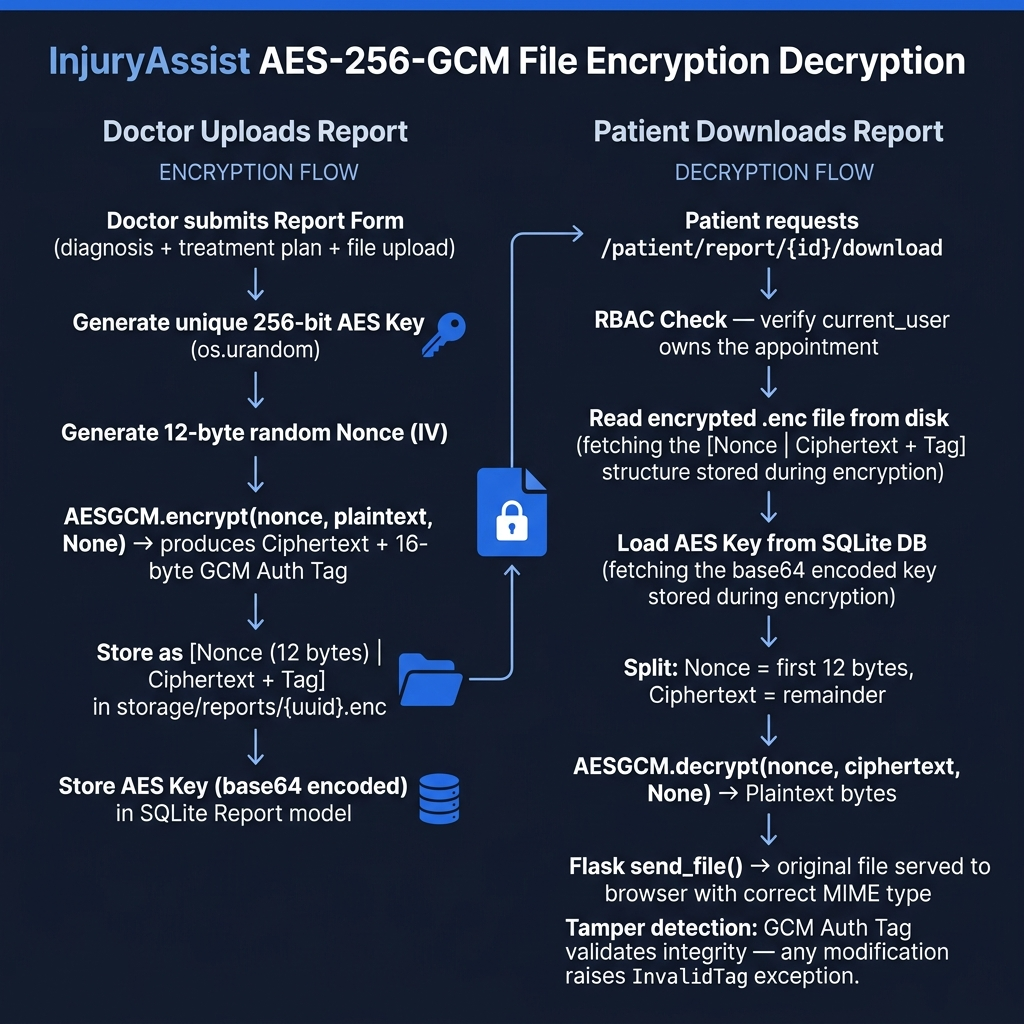
\includegraphics[width=0.9\textwidth]{encryption_flow.png}
        \end{modelbox}
    \end{minipage}
    \hfill
    \begin{minipage}{0.48\textwidth}
        \begin{modelbox}{Authentication Workflow}
            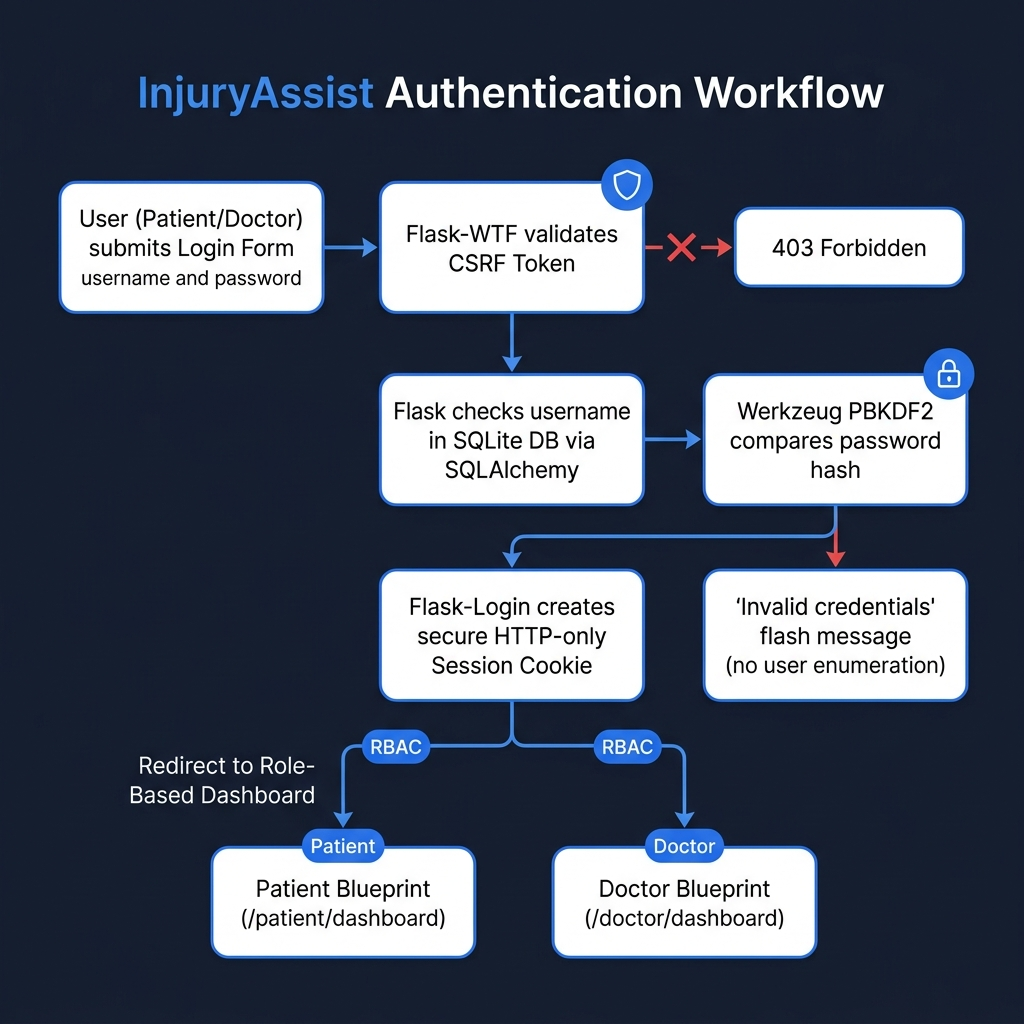
\includegraphics[width=0.9\textwidth]{auth_flow.png}
        \end{modelbox}
    \end{minipage}
\end{figure}

\section{Appendix}
\textbf{Glossary:} AES-256-GCM (Advanced Encryption Standard Galois/Counter Mode), RBAC (Role-Based Access Control), CSRF (Cross-Site Request Forgery), PBKDF2 (Password-Based Key Derivation Function 2). \\

\end{document}
